\documentclass{article}
\usepackage[utf8]{inputenc}
\usepackage[letterpaper, margin=2.5cm]{geometry}
\usepackage[euler-digits, euler-hat-accent]{eulervm}
\usepackage{amsmath, amsthm, amsfonts, amssymb}
\usepackage{graphicx}
\usepackage[framemethod=tikz]{mdframed}
\usepackage{enumitem}
\usepackage{wasysym}
\usepackage{tikz}
\usepackage{array}
\usepackage{epigraph}
\usepackage{caption}
\usepackage{algorithm}
\usepackage[noend]{algpseudocode}

\usetikzlibrary{decorations.pathmorphing}

\newtheorem{theorem}{Theorem}

\newcommand{\nameditem}[1]{\item\textbf{#1}}
\newcommand{\impl}{\item[$\Rightarrow$]}

\newcommand{\NTIME}{\ensuremath{\textsf{NTIME}}}
\newcommand{\Poly}{\ensuremath{\textsf{P}}}
\newcommand{\NP}{\ensuremath{\textsf{NP}}}
\newcommand{\NEXP}{\ensuremath{\textsf{NEXP}}}
\newcommand{\NEXPEXP}{\ensuremath{\textsf{NEXPEXP}}}
\newcommand{\coNP}{\ensuremath{\textsf{coNP}}}
\newcommand{\coNEXP}{\ensuremath{\textsf{coNEXP}}}
\newcommand{\coNEXPEXP}{\ensuremath{\textsf{coNEXPEXP}}}
\newcommand{\interP}{\ensuremath{\textsf{NP}\cap\textsf{coNP}}}
\newcommand{\interEXP}{\ensuremath{\textsf{NEXP}\cap\textsf{coNEXP}}}
\newcommand{\interEXPEXP}{\ensuremath{\textsf{NEXPEXP}\cap\textsf{coNEXPEXP}}}
\newcommand{\unionP}{\ensuremath{\textsf{NP}\cup\textsf{coNP}}}
\newcommand{\unionEXP}{\ensuremath{\textsf{NEXP}\cup\textsf{coNEXP}}}
\newcommand{\unionEXPEXP}{\ensuremath{\textsf{NEXPEXP}\cup\textsf{coNEXPEXP}}}

% zigzag arrows
\newlength{\LETTERheight}
\AtBeginDocument{\settoheight{\LETTERheight}{I}}
\newcommand*{\longleadsto}[1]{\ \raisebox{0.24\LETTERheight}{\tikz \draw [->,
line join=round,
decorate, decoration={
    zigzag,
    segment length=4,
    amplitude=.9,
    post=lineto,
    post length=2pt
}] (0,0) -- (#1,0);}\ }

% thick lines in the Bingo sheet
\makeatletter
\newcommand{\thickhline}{%
    \noalign {\ifnum 0=`}\fi \hrule height 1pt
    \futurelet \reserved@a \@xhline
}
\newcolumntype{"}{@{\hskip\tabcolsep\vrule width 1pt\hskip\tabcolsep}}
\makeatother

\renewcommand\thetheorem{\Roman{theorem}}

\newcounter{exercise}
\newenvironment{exercise}[1][]{\refstepcounter{exercise}\par\medskip\noindent\textbf{Exercise~\theexercise.#1} \rmfamily}{\medskip}

\setlist[description]{topsep=1pt, itemsep=1pt, leftmargin=0.5cm}
\setlist[itemize]{topsep=1pt, itemsep=1pt}

% prevents "then" and "do" clutter in the pseudo code
\renewcommand\algorithmicthen{}
\renewcommand\algorithmicdo{}

\begin{document}

\title{The Nondeterministic Time Hierarchy}
\author{Sebastian Oberhoff\\{\small oberhoff.sebastian@gmail.com}}
\date{\today}

\maketitle

\begin{abstract}
\begin{center}
Let's play some Bingo. Here's our card:\medskip

\begin{tabular}{|c"c|c|c|c|}
\hline
& \NEXP & \coNEXP & \interEXP & \unionEXP\\\thickhline
\NP & & & & \\\hline
\coNP & & & & \\\hline
\interP & & & & \\\hline
\unionP & & & & \\\hline
\end{tabular}\medskip

Using simple brute force all the classes on the left are contained in those at the top. But are these containments strict? That's the challenge. To put a ``$\subsetneq$" in every spot. Hold on to your potatoes.
\end{center}
\end{abstract}

\setlength{\epigraphwidth}{\textwidth}

\epigraph{I find that if I just sit down and think... the solution presents itself.}{\textit{Professor Henry Jones Sr.}}

\begin{figure}[h]
\centering
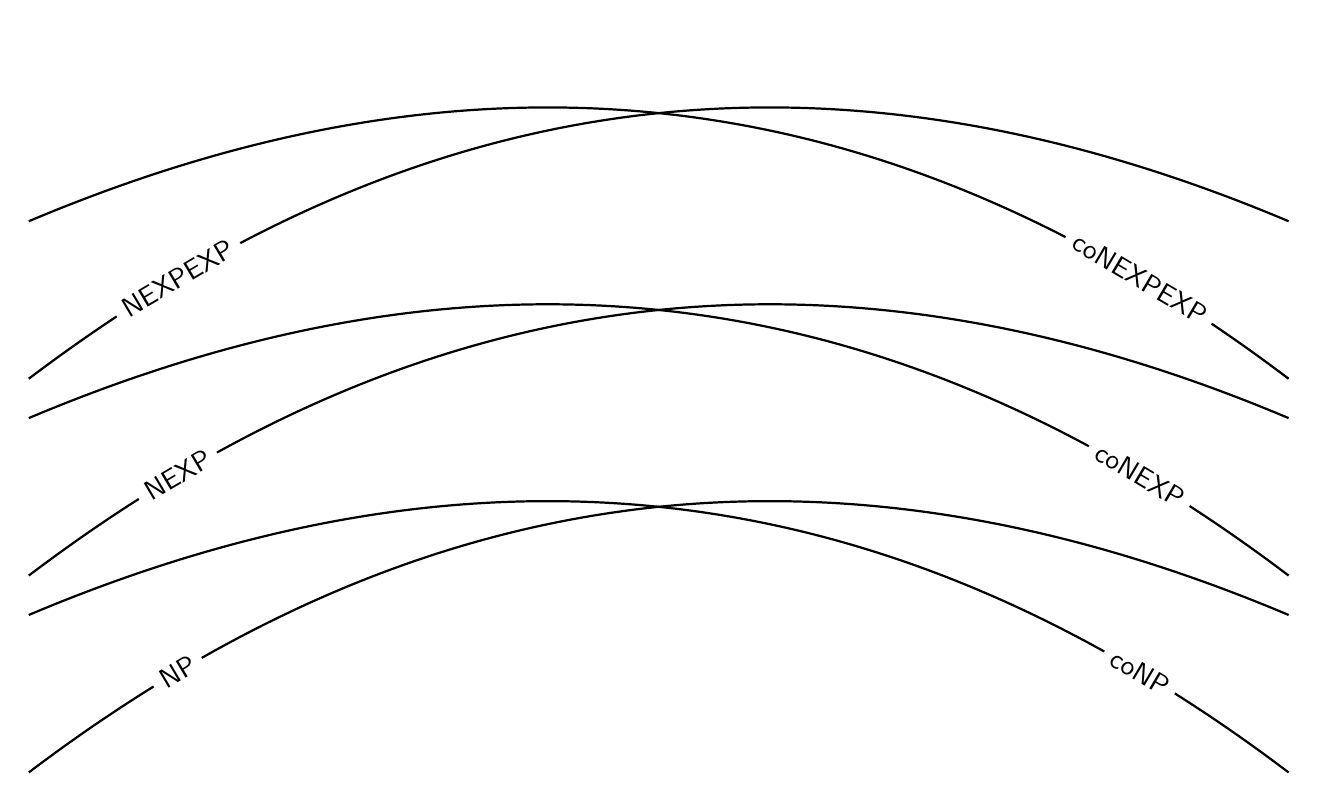
\begin{tikzpicture}
\draw[thick] (-8, 0) to[bend left] node[very near start, sloped, fill=white] {$\NP$} (8, 2);
\draw[thick] (8, 0) to[bend right] node[very near start, sloped, fill=white] {$\coNP$} (-8, 2);
\draw[thick] (-8, 2.5) to[bend left] node[very near start, sloped, fill=white] {$\NEXP$} (8, 4.5);
\draw[thick] (8, 2.5) to[bend right] node[very near start, sloped, fill=white] {$\coNEXP$} (-8, 4.5);
\draw[thick] (-8, 5) to[bend left] node[very near start, sloped, fill=white] {$\NEXPEXP$} (8, 7);
\draw[thick] (8, 5) to[bend right] node[very near start, sloped, fill=white] {$\coNEXPEXP$} (-8, 7);
\end{tikzpicture}
\caption{The Nondeterministic Time Hierarchy.}
\end{figure}

\section{``Se\~{n}or, Nobody's Come Out Of There Alive."}

\begin{theorem}
$\NP \subsetneq \NEXP$.
\end{theorem}

\begin{proof}
Let's start by contemplating the following problem:
\begin{mdframed}
\textsc{NCatch22}$^n$
\begin{itemize}[noitemsep,topsep=0.3em]
\item[$\longrightarrow$] A nondeterministic algorithm $N$.
\item[$\longrightarrow$] An integer $t$ in unary.
\end{itemize}
\begin{itemize}[noitemsep,topsep=0.3em]
\item[$\longleftarrow$] Accept if there's no path of execution such that $N(N, t)$ accepts within $2^n$ steps.\footnotemark\ Reject otherwise.
\end{itemize}
\end{mdframed}
\footnotetext{As is customary, $n$ is the size of the input.}
On the one hand, we can solve this problem in deterministic doubly exponential time by just going through all possible lines of execution. This is true even if $N$ varies, not just $t$. Increasing the size of the source code of $N$ isn't \textit{that} catastrophic. So if we give ourselves an expexporbitant budget, we're good. That puts the problem in \textsf{EXPEXP} and thereby in $\NEXPEXP$.

On the other hand, suppose for a moment that we could somehow solve this problem in $f(n) \in o(2^n)$ steps with some nondeterministic algorithm $N^*$. Any such algorithm could be turned back around on itself by asking whether there exists a path of execution such that $N^*(N^*, t)$ accepts within $2^n$ steps. Let $t$ be large enough so that $f(n) \ll 2^n$, then:\\[0.5em]
\begin{minipage}{0.35\textwidth}
\begin{description}[noitemsep]
\nameditem{Either there is such a path:} 
\begin{itemize}[noitemsep]
\impl $N^*(N^*, t)$ always rejects.
\impl There is no such a path. \lightning
\end{itemize}
\end{description}
\end{minipage}
\begin{minipage}{0.5\textwidth}
\begin{description}[noitemsep]
\nameditem{Or there is no such path:} 
\begin{itemize}[noitemsep]
\impl $N^*(N^*, t)$ \textit{someway} accepts within $f(n)$ steps.
\impl There is such a path. \lightning
\end{itemize}
\end{description}
\end{minipage}\\[1em]
As we can see, it's impossible for any nondeterministic algorithm to accomplish this task in $o(2^n)$ steps. In particular, because $O\left(2^{n/2}\right) \subseteq o(2^n)$, it's impossible to accomplish this task in $\NTIME\left(2^{n/2}\right)$. And since this class contains all of nondeterministic polynomial time we have
\[
\NP \subseteq \NTIME\left(2^{n/2}\right) \subsetneq \NEXPEXP\,.
\]
Just one small problem. That's one ``\textsf{EXP}" too many. Dang it!

At this point the classical route is to start over and try something cleverer instead: lazy diagonalization.\cite{stanislav} Certainly, that's the way to go if you want to squeeze out the best possible Nondeterministic Time Hierarchy Theorem. But we're not here for elaborately choreographed sword fights. We're here to cleave the polynomial and the exponential apart. So let's just shoot the sucker.

Imagine $\NP = \NEXP$. Then $\NEXP = \NEXPEXP$. How so? \textit{Padding}, that's how. Therefore, by chaining our equalities we get $\NP = \NEXP = \NEXPEXP$. And we know this isn't true. QED.

All that's left over is to double check the details involved in the padding. For this take any problem in $\NEXPEXP$. Then there exists a nondeterministic algorithm $J$ which can take an $n$ bit input and accept within $2^{2^{n^k}}$ steps for some $k \in \mathbb{N}$, provided the input is a ``yes"-instance. Here's an illustration:
\[
\overbrace{\text{\footnotesize Only the penitent man will pass.}}^{n\text{ bits}}\overset{2^{2^{n^k}}\text{ nondeterministic steps}}{\longleadsto{4}} \text{\footnotesize He kneels!}
\]
If we pad this input, we get a similar problem:
\[
\underbrace{\overbrace{\text{\footnotesize Only the penitent man will pass.}}^{n\text{ bits}}\overbrace{\text{\footnotesize BLABLABLABLABLABLABLABLABLABLA...}}^{\text{An entire book}}}_{2^{n^k}\text{ bits}}\overset{2^{2^{n^k}}\text{ nondeterministic steps}}{\longleadsto{4}} \text{\footnotesize He kneels!}
\]
Since $J$ solves the former in $2^{2^{n^k}}$ steps we can easily modify it to ignore the padding and still solve the latter in $2^{2^{n^k}}$ steps. But this problem now has a size $m = 2^{n^k}$ input. In other words, we can solve the latter problem in $2^m$ steps which now is merely exponential in the size of the input. Therefore, as long as $\NP = \NEXP$, we can also solve the latter problem in $m^l$ steps for some $l\in\mathbb{N}$ using some new algorithm $J'$. And that gives us the following algorithm:
\begin{enumerate}
\item Take the $n$ bit input and pad it to length $2^{n^k}$. (And return to the starting position.)
\item Jump to the initial state of $J'$ and run it for the remainder of the computation. 
\end{enumerate}
The first stage takes $O\left(2^{n^k}\right)$ time. The second takes $m^l = \left(2^{n^k}\right)^l = 2^{ln^k}$ time. That's exponential in total. So we've arrived in the promised land: $\NEXP$.
\end{proof}

We have our first separation. And we've added the first of two weapons we'll be using to our belt: padding. Using it and diagonalization we're now equipped to climb the hierarchy.

\begin{exercise}
Which steps in the above proof need to be modified in order to establish $\NEXP \subsetneq \NEXPEXP$?
\end{exercise}

Alright, time to fetch the other weapon.

\begin{theorem}
$\coNP \subsetneq \coNEXP$.
\end{theorem}

It would be quite the hassle if we had to start over. Fortunately, we don't have to. We can simply argue by \textit{symmetry} instead.

\begin{proof}
Suppose $\coNP = \coNEXP$. Then we could prove $\NP = \NEXP$ which we know to be false. This works like so: Take an arbitrary problem in $\NEXP$ and simply interchange the ``yes" and ``no" labels. Now it's a problem in $\coNEXP$ making it a problem in $\coNP$. But that means the unmodified problem is in $\NP$. \lightning
\end{proof}

\section{``Hang On Lady. We're Going For A Ride."}

Time to check our Bingo card.
\begin{center}
\begin{tabular}{|c"c|c|c|c|}
\hline
& \NEXP & \coNEXP & \interEXP & \unionEXP\\\thickhline
\NP & $\subsetneq$ & & & $\subsetneq$ \\\hline
\coNP & & $\subsetneq$ & & $\subsetneq$ \\\hline
\interP & $\subsetneq$ & $\subsetneq$ & & $\subsetneq$ \\\hline
\unionP & & & & \\\hline
\end{tabular}
\end{center}
I took the liberty of adding some entries that are trivial consequences. Now for the merely elementary consequences. I recommend mentally following along with Figure 1 as you read these.

\begin{theorem}
$\NP\subsetneq\coNEXP$.
\end{theorem}

\begin{proof}
If
\[
\NP = \coNEXP,
\]
then
\[
\coNP = \NEXP
\]
by symmetry. Hence, by Theorem I and II, $\NP$ and $\coNP$ strictly contain each other. \lightning
\end{proof}

\begin{theorem}
$\coNP\subsetneq\NEXP$.
\end{theorem}

\begin{proof}
By the previous theorem and symmetry.
\end{proof}

\begin{theorem}
$\interP \subsetneq \interEXP$.
\end{theorem}

\begin{proof}
\[
\begin{aligned}
\interP & \subseteq \NP & & \text{(duh)}\\
& \subsetneq \NEXP & & \text{(by Theorem 1)}\\
& \subseteq \interEXPEXP & & \text{(by brute force)}
\end{aligned}
\]
Now suppose
\[
\interP = \interEXP.
\]
Then
\[
\interEXP = \interEXPEXP
\]
by padding. Hence,
\[
\interP = \interEXPEXP
\]
which we've just observed to be untrue. \lightning
\end{proof}

\begin{theorem}
$\NP \subsetneq \interEXP$.
\end{theorem}

\begin{proof}
If
\[
\NP = \interEXP,
\]
then
\[
\coNP = \interEXP
\]
by symmetry. Hence, 
\[
\NP = \coNP = \interP\footnote{If two sets are equal, then intersecting them yields the same set again.} = \interEXP.
\]
But this is ruled out by the previous theorem. \lightning
\end{proof}

\begin{theorem}
$\coNP \subsetneq \interEXP$.
\end{theorem}

\begin{proof}
By the previous theorem and symmetry.
\end{proof}

\begin{theorem}
$\unionP \subsetneq \NEXP$.
\end{theorem}

\begin{proof}
If
\[
\unionP = \NEXP,
\]
then
\[
\unionP = \coNEXP
\]
by symmetry. Furthermore,
\[
\unionEXP = \NEXPEXP
\]
by padding. Putting all this together we then get
\[
\NEXP = \coNEXP = \unionEXP\footnote{Again, if two sets are equal, their union is unchanged.} = \NEXPEXP.
\]
And that contradicts the conclusion of the first exercise. \lightning
\end{proof}

\begin{theorem}
$\unionP \subsetneq \coNEXP$.
\end{theorem}

\begin{proof}
By the previous theorem and symmetry.
\end{proof}

Marion: ``Well Jones, at least you haven't forgotten how to show a lady a good time!"

\begin{exercise}
Imagine standing in front of a black board with Figure 1 on it and saying: ``If that is that, then that is also that. Hence, that equals that equals that equals that. But that \textit{isn't} equal to that. Contradiction." Which theorem have you just established?
\end{exercise}

\begin{exercise}
Find an alternate proof of Theorem III which doesn't rely on two sets strictly containing each other.
\end{exercise}

\section{``Where's The Ten?"}
This is where we're at:
\begin{center}
\begin{tabular}{|c"c|c|c|c|}
\hline
& \NEXP & \coNEXP & \interEXP & \unionEXP\\\thickhline
\NP & $\subsetneq$ & $\subsetneq$ & $\subsetneq$ & $\subsetneq$ \\\hline
\coNP & $\subsetneq$ & $\subsetneq$ & $\subsetneq$ & $\subsetneq$ \\\hline
\interP & $\subsetneq$ & $\subsetneq$ & $\subsetneq$ & $\subsetneq$ \\\hline
\unionP & $\subsetneq$ & $\subsetneq$ & & $\subsetneq$ \\\hline
\end{tabular}
\end{center}
Only one more to go. And this is the main villain. While $\unionP$ is the ``biggest" set on the polynomial level $\interEXP$ is the ``smallest" set on the exponential level. It doesn't get any closer. Moreover, upon reflection it becomes apparent that every other theorem we've proven so far immediately follows from this one. If we had proven this one first, we could've stopped right there. But that would've been way less fun. And we need to fill our running time somehow, right? Anyway, this one's surely going to be just another pushover. We all but made it.

Dr. Jones Sr.: ``When we're airborne, with Germany behind us, then I'll share that sentiment."

At first, one might almost reflexively think that, hey, we've proven both $\NP \subsetneq \interEXP$ and $\coNP \subsetneq \interEXP$. So we're immediately done. But if one thinks about this for just two more seconds, one realizes that this isn't even close to enough. Maybe $\NP$ is the ``left half" of $\interEXP$ and $\coNP$ is the ``right half" (with some overlap).

Fine, let's use our whip then. Suppose $\unionP = \interEXP$. Then by symmetry we get... squat. Nothing happened at all. What if we try the gun? Sure, we could deduce $\unionEXP = \interEXPEXP$. Then what? These puzzle pieces don't fit together.

Indiana: ``Willie! Willie, we're in trouble!"

Things are indeed dire. Padding and symmetry could only bring us so far. We're going to need a new idea. So here's one: If we think back to Theorem VIII where we established $\unionP \subsetneq \NEXP$, there was an alternative proof available. We could've \textit{exhibited} a single problem in $\NEXP$ and shown that this problem is neither in $\NP$ nor $\coNP$. Thereby, it isn't in $\unionP$. What might such a problem be? An $\NEXP$-complete problem of course!\footnote{Let's not worry too much about what kind of reductions we'd allow.} Such a problem is in $\NEXP$ and if it is in either $\NP$ or $\coNP$, then the classes collapse. And that can't happen.

Cool. So all we need is an $\interEXP$-complete problem, right? Sure, that would do it. Unfortunately, this is a little tricky. We don't even have $\interP$-complete problems. And believe me people have definitely been looking. But then what hope is there to find an $\interEXP$-complete problem?

Marion: ``Where are you going?"

Indiana: ``Through that wall."

To overcome this problem let's go back a couple steps to before we thought of using complete problems. All we said at that point is that we need some problem which is neither in $\NP$ nor in $\coNP$. Can we cook up something else that fits this bill? Scanning over the theorems we have so far, the best we can do is to use Theorem VI to produce some problem in $\interEXP$ which isn't in $\NP$. And we can use Theorem VII to produce another which isn't in $\coNP$. But we have no way of knowing if these are the same problem. Can we fix this? Sorta. We're going to have to go between them.

Elsa: ``Go between them? Are you crazy?!"

In 1975 Richard E. Ladner proved a remarkable theorem known today as Ladner's Theorem.\cite{ladner} This theorem establishes that if, as we all expect, $\Poly \subsetneq \NP$, then there are problems in $\NP$ which are neither in $\Poly$ nor $\NP$-complete. They are ``between" $\Poly$ and $\NP$-complete. The way Ladner did this was to argue:

\noindent
``Suppose $\Poly \subsetneq \NP$. Then give me:
\begin{itemize}
\item A problem in $\NP$ that isn't in $\Poly$. Because $\Poly \subsetneq \NP$ any $\NP$-complete problem will do.
\item A problem in $\NP$ that isn't $\NP$-complete. Because $\Poly \subsetneq \NP$ any problem in $\Poly$ will do.
\end{itemize}
Given these two problems you can mash them together like so and produce a new problem that's still in $\NP$ but which is neither in $\Poly$ nor is $\NP$-complete."

Now that sounds like exactly what the doctor ordered. We have a problem in $\interEXP$ that isn't in $\NP$. And we have another that isn't in $\coNP$. Let's mash 'em together!

\begin{theorem}
$\unionP \subsetneq \interEXP$.
\end{theorem}

\begin{proof}
By Theorems VI and VII we're guaranteed the existence of languages $E$ and $A$ which aren't in $\NP$ and $\coNP$ respectively,\footnote{I chose the letters $E$ and $A$ because they harken back to the definitions of $\NP$ and $\coNP$ that use $\exists$ and $\forall$ quantifiers. The fact that they're reversed compared to the quantifiers can be used as a reminder that $E$ is \textit{not} in $\NP$ and $A$ is \textit{not} in $\coNP$.} yet which are in $\interEXP$. Now consider the language $\AE$ defined as follows:
\[
\AE(x) =
\begin{cases}
E(x) & \text{if $f(|x|)$ is even}\\
A(x) & \text{if $f(|x|)$ is odd.}\\
\end{cases}
\]
where $f$ is defined as:
\begin{algorithm}[H]
\caption*{$f(n)$}
\begin{algorithmic}
\If{$n = 0$}
  \State \Return{$0$}
\EndIf
\If{$f(n-1) = 2i$ for some $i \in \mathbb{N}$}
  \While{$n$ steps have not yet elapsed}
    \For{$x \in$ all possible strings}
      \If{$\AE(x) \subsetneq N_i(x)$ \textbf{or} $N_i(x)$ takes too long on a ``yes"-instance}
        \State \Return{$f(n-1)+1$}
      \EndIf
    \EndFor
  \EndWhile
  \State \Return{$f(n-1)$}
\EndIf
\If{$f(n-1) = 2i+1$ for some $i \in \mathbb{N}$}
  \While{$n$ steps have not yet elapsed}
    \For{$x \in$ all possible strings}
      \If{$\AE(x) \subsetneq N_i(x)$ \textbf{or} $N_i(x)$ takes too long on a ``no"-instance}
        \State \Return{$f(n-1)+1$}
      \EndIf
    \EndFor
  \EndWhile
  \State \Return{$f(n-1)$}
\EndIf
\end{algorithmic}
\end{algorithm}
\noindent
This code warrants some comments.
\begin{description}
\nameditem{What's going on with these while-statements?} These statements run the nested code for the specified amount of time. If it returns by then, fine. But if it doesn't, it is aborted and the following \textbf{return}-statement on the same level is executed. This hard time limit assures that $f$ can be computed in roughly $T(n) = T(n-1) + n$ steps for some function $T$. That's a mere quadratic amount; very manageable.\footnote{I'm sweeping the issue of keeping track of time under the rug. It should be clear though that this doesn't endanger our polynomial budget. (In fact, since we're not operating under Ladner's constraints, we even have an exponential budget.)}
\begin{description}
\nameditem{What's happening \textit{inside} these while-blocks?} Let's just take the first of these. Here we're taking the $i$'th polynomial time nondeterministic algorithm ($N_i$) and checking it against $\AE$. We could try to speed this up by using nondeterminism ourselves. But as it turns out we don't need to. So we're free to assume that everything here is brute forced in deterministic fashion. What we're doing here is we're looking to disprove the assertion that $\AE$ is in $\NP$ by looking for counterexamples ruling out every possible $N_i$. That just leaves two subtle subproblems.
\begin{description}
\nameditem{How can we figure out \AE$(x)$ if \AE\ is defined in terms of $f$ again? Isn't this circular?} Not quite. What saves us is that in order to determine the relevant values of $\AE(x)$ we only need to know $f$ for much smaller values. Remember that we only run this loop for $n$ steps. At that point we can only have reached $x$'s of at most logarithmic size. This in turn only demands $\AE$ and thereby $f$ to be defined up to logarithmic size. So, as long as we operate recursively---and we already do for $f(n-1)$---we're in the clear.
\nameditem{How do we actually make a list of all the \textit{polynomial time} nondeterministic algorithms?} This sounds like a formidable task. And it is. But luckily there's a way to sidestep it. We simply have to demand that each $N_i$ comes with a header which declares its running time. All we have to do then is check the header and make sure that $N_i$ doesn't overstep its bounds. If it does, we increment $f$ and move on. As we'll see this measure is fully sufficient.
\end{description}
\end{description}
\end{description}
With all that out of the way we're now ready for the key questions.
\begin{description}
\nameditem{Is \AE\ in $\interEXP$?} Both $E$ and $A$ are. So, for example, we can accept ``yes"-instances in $\NEXP$ time by first computing $f(|x|)$---that takes a mere polynomial amount---and then jumping to the appropriate $\NEXP$ algorithm depending on whether $f(|x|)$ is even or odd. The same is true for ``no"-instances. \checkmark
\nameditem{And finally, is \AE\ in either $\NP$ or $\coNP$?} Let's assume that it is. Then, without loss of generality, let $N^*$ be the ``first" algorithm affirming this assumption by placing $\AE$ in $\NP$. This would mean that, as we consider larger and larger inputs, $f$ discards every nondeterministic algorithm until it eventually reaches $N^*$. At that point it gets stuck. Because $N^*$ answers correctly to every input, and does so for the ``yes"-instances within a polynomial time limit, $f$ will never grow to the next higher number. Hence, $f$ is even for all but a finite number of inputs. Hence, $\AE$ is equal to $E$ for all but a finite number of strings. Hence, by solving $\AE$, $N^*$ solves $E$ on all but a finite number of inputs; placing $E$ in $\NP$. Hence, $N^*$ couldn't have existed after all. \lightning
\end{description}
\end{proof}

Indiana: ``X marks the spot... Bingo."\footnote{Finally, the purpose of the Roman numerals is revealed.}

\begin{thebibliography}{2}
\bibitem{stanislav}
Žák Stanislav (1983), \textit{A Turing machine time hierarchy, Theoretical Computer Science, Elsevier Science B.V. 26}
\bibitem{ladner}
Richard E. Ladner (1975), \textit{On the Structure of Polynomial Time Reducibility, Journal of the ACM}
\end{thebibliography}

\vfill\eject

\end{document}